\section{Введение}

\subsection{Цель работы}

Изучение фундаментальных законов механики лежит в основе классической физики. Одним из важнейших принципов, подтверждаемых экспериментально, является принцип эквивалентности инертной и гравитационной массы. Согласно этому принципу, все тела в однородном гравитационном поле Земли падают с одинаковым ускорением вне зависимости от их массы и состава.

В данной лабораторной работе рассматривается свободное падение тел и проводится экспериментальная проверка указанного принципа. Основной задачей является измерение ускорения свободного падения при помощи частотомера-хронометра Ч3-32, который позволяет с высокой точностью фиксировать интервалы времени между двумя последовательными событиями. Это устройство является удобным инструментом для анализа быстропротекающих процессов и широко используется в учебной и исследовательской практике.

Кроме того, в ходе работы проводится анализ точности измерений и определение погрешностей, что позволяет оценить достоверность полученных результатов. Особое внимание уделяется вычислению погрешностей при косвенных измерениях, поскольку именно такие данные наиболее часто встречаются в физическом эксперименте.


\subsection{Решаемые задачи}
\begin{enumerate}
    \item Проверка принципа эквивалентности масс.
    \item Измерение ускорения свободного падения тел.
    \item Знакомство с методом измерения интервалов времени между импульсами частотомером – хронометром Ч3-32.
    \item Определение погрешности косвенных измерений.
\end{enumerate}

\section{Основная часть}

\subsection{Теоретическая часть}
Если справедлив принцип эквивалентности, то время пролета участка при
свободном падении тел различной массы (при одинаковых условиях) будет одинаково.
Экспериментальная проверка этого факта и является целью настоящей работы.

Как известно, уравнение движения тела при свободном падении имеет вид:
\begin{equation}
h = v_0 t + \frac{1}{2} g t^2, \label{eq:fall}
\end{equation}
где \( v_0 \) — начальная скорость шарика при подходе к верхнему лучу (указана на установке),  
\( t \) — время падения, \( g \) — ускорение свободного падения, \( h \) — пройденный путь.

Отсюда выражаем ускорение свободного падения:
\[
g = \frac{2(h - v_0 t)}{t^2}
\]
при \( v_0 = 1{,}050 \pm 0{,}005 \, \text{м/с} \) — начальная скорость шарика, 
\( h = 0{,}272 \pm 0{,}001 \, \text{м} \) — расстояние между лучами, 
\( t \) — среднее время падения.


Погрешность измерения времени вычисляется по формуле:

\begin{equation}
\Delta t = \sqrt{ \frac{\sum d_i^2}{n(n - 1)} },
\end{equation}

где \( n \) — число измерений, а \( d_i \) — отклонения отдельных измерений от среднего значения.

Погрешность измерения ускорения свободного падения рассчитывается по формуле:

\[
\Delta g = \sqrt{ 
\frac{1}{9} \left( \frac{\partial g}{\partial h} \right)^2 \Delta h^2 +
\frac{1}{9} \left( \frac{\partial g}{\partial v_0} \right)^2 \Delta v_0^2 +
\left( \frac{\partial g}{\partial t} \right)^2 \Delta t^2
}
\]

где производные берутся от выражения:
\[
g = \frac{2(h - v_0 t)}{t^2}
\]

После подстановки производных и значений, выражение принимает вид:
\[
\Delta g = 2 \cdot \sqrt{
\frac{1}{9} \left( \frac{1}{t^2} \right)^2 \cdot (0{,}001)^2 +
\frac{1}{9} \left( \frac{1}{t} \right)^2 \cdot (0{,}005)^2 +
\left( \frac{v_0 t - 2h}{t^3} \right)^2 \cdot \Delta t^2
}
\, \text{м/с}^2
\]

При выполнении эксперимента присутствовали источники систематических ошибок, такие как сопротивление воздуха, которое действовало по-разному на разные шарики в виду того, что их масса и материал поверхности неодинаковы.

\subsection{Эксперимент}
Схема установки приведена на рисунке. 
Луч от квантового генератора ЛГ направляется на призму полного внутреннего отражения П1, от нее на призму П2, а затем на фотодиод ФД. 
При отодвигании заслонки З шарик, находящийся в трубке Т, падает в лузу Л и пересекает два световых луча, расстояние между которыми равно h . Когда шарик пересекает верхний луч, фотодиод ФД вырабатывает импульс, который усилившись в усилителе, подается на вход частотомера Ч3-32 и запускает его. 
При пересечении шариком нижнего луча импульс от фотодиода останавливает счет
частотомера. 
Интервал времени между двумя импульсами, регистрируемый
частотомером, равен времени пролета t шарика от верхнего луча до нижнего. Усилитель питается от источника УПУ-1У4.

\begin{figure}[H]
\centering
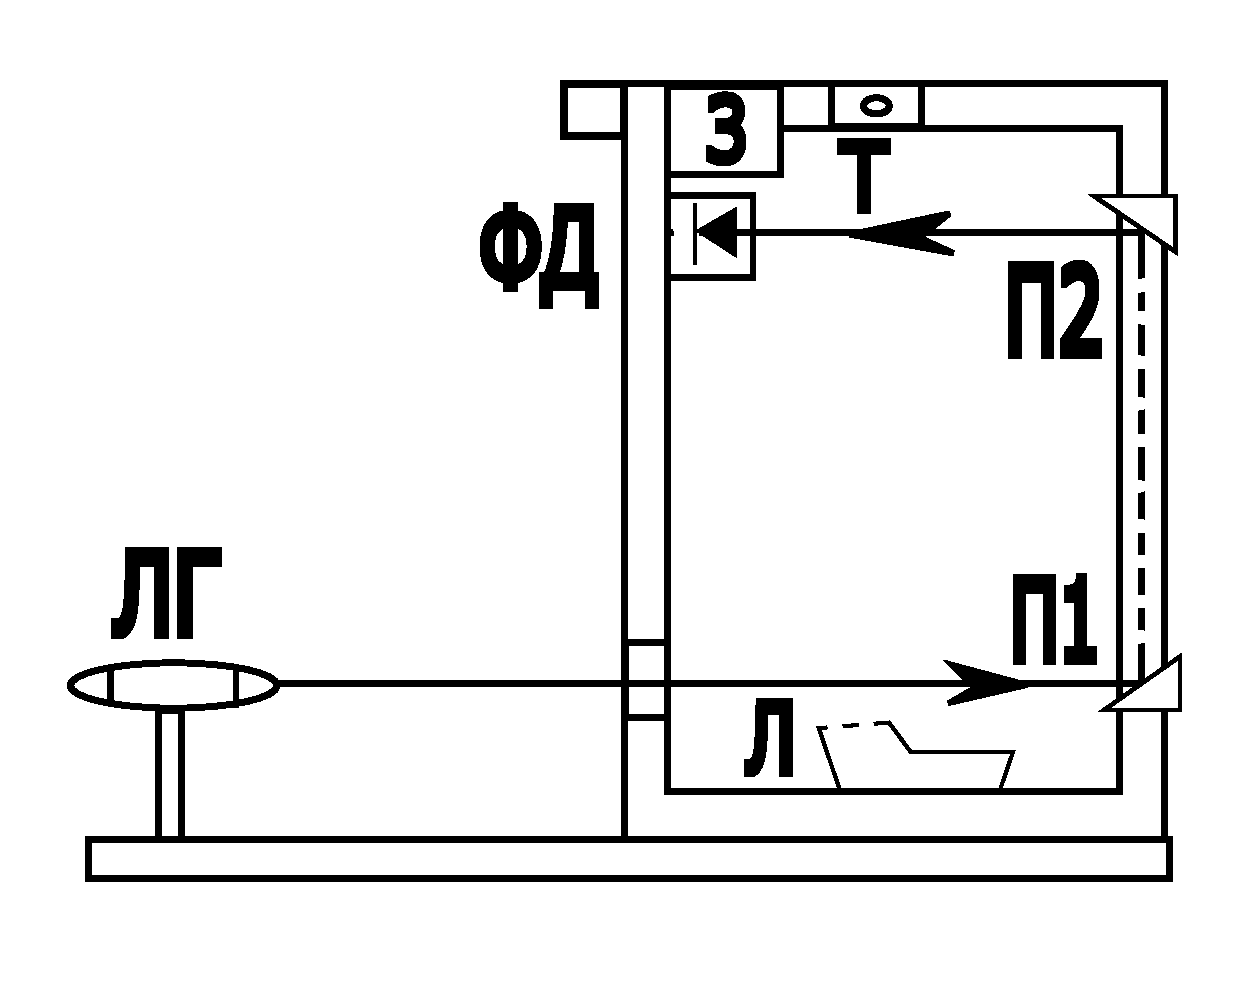
\includegraphics[width=0.8\textwidth]{схема лазера.pdf}

\caption{Схема установки}
\label{fig:sketch}
\end{figure}

\begin{figure}[H]
\centering
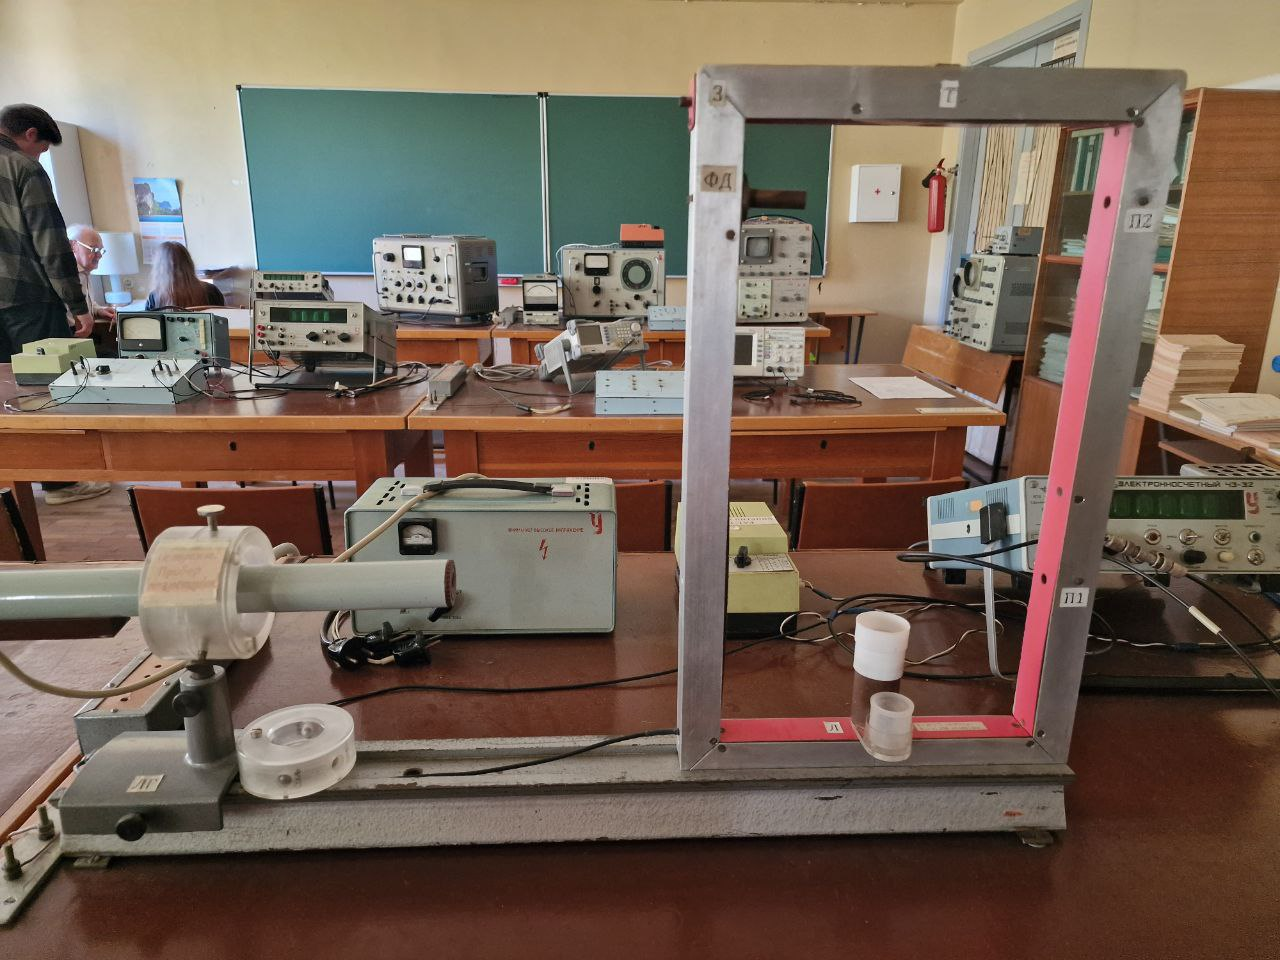
\includegraphics[width=0.6\textwidth]{photo_2025-06-02_04-35-33.jpg}
\caption{Фотография установки}
\label{fig:device}
\end{figure}


\subsection{Обработка данных и обсуждение результатов}
Для написания программы, вычисляющей все требуемые данные, используется язык C++; среда разработки - Visual Studio.
Код полностью расположен в репозитории на GitHub.
Сначала рассчитаем среднее время падения шариков различных материалов:
\subsubsection{Исходный код} 

\begin{lstlisting}[label=listing1, caption=Функция для вычисления стандартного отклонения]
double standardDeviation(const vector<double>& data, double mean) {
    double sumOfSquaredDifferences = 0.0;
    for (double value : data) {
        sumOfSquaredDifferences += pow(value - mean, 2);
    }
    return sqrt(sumOfSquaredDifferences / (data.size() - 1));
}

double calculateError(double stdDev, int numMeasurements) {
    return stdDev / sqrt(numMeasurements);
}

\end{lstlisting}


\begin{lstlisting}[label=listing1, caption=Функция для вычисления массы шариков]
double standardDeviation(const vector<double>& data, double mean) {
    double sumOfSquaredDifferences = 0.0;
    for (double value : data) {
        sumOfSquaredDifferences += pow(value - mean, 2);
    }
    return sqrt(sumOfSquaredDifferences / (data.size() - 1));
}

double calculateError(double stdDev, int numMeasurements) {
    return stdDev / sqrt(numMeasurements);
}
\end{lstlisting}

\begin{lstlisting}[label=listing1, caption=Функция для вычисления погрешности времени]
 for (int j = 0; j < 6; ++j) {
        double sum = 0.0;
        for (int i = 0; i < n; ++i) {
            sum += timeData[i][j];
        }
        double mean = sum / n;

        double sq_sum = 0.0;
        for (int i = 0; i < n; ++i) {
            sq_sum += pow(timeData[i][j] - mean, 2);
        }
        double stdev = sqrt(sq_sum / (n * (n - 1)));

        std::cout << "| " << std::setw(11) << substances[j] << " | "
            << std::setw(19) << mean << " | "
            << std::setw(16) << stdev << " |" << std::endl;
\end{lstlisting}

\begin{lstlisting}[label=listing1, caption=Функция для вычисления ускорения свободного падения]
vector<string> substance_names = { "Алюминий", "Латунь", "Сталь", "Дерево", "Плексиглас", "Свинец" };
    vector<double> g_values(substance_names.size());
    vector<double> t_values(substance_names.size());

    double h = 0.272; // м
    double h_error = 0.001; // м
    double v = 1.050; // м/с
    double v_error = 0.005; // м/с

    for (size_t i = 0; i < substance_names.size(); ++i) {
        double sum = 0.0;
        for (size_t j = 0; j < fall_times_ms.size(); ++j) {
            sum += fall_times_ms[j][i];
        }
        double t_ms = sum / fall_times_ms.size();
        double t = t_ms / 1000.0;               
        t_values[i] = t;

        g_values[i] = (2 * (h - v * t)) / (t * t);
    }
\end{lstlisting}

\begin{lstlisting}[label=listing1, caption=Функция для вычисления погрешности ускорения свободного падения]
        double dt = 0.000001;
        double term1 = (1.0 / 9.0) * pow(1.0 / (t * t), 2) * pow(h_error, 2);
        double term2 = (1.0 / 9.0) * pow(1.0 / t, 2) * pow(v0_error, 2); // Use v0_error instead of v_error
        double term3 = pow(((v0 * t - 2 * h) / (t * t * t)), 2) * pow(dt, 2); // Use v0 instead of v

        g_errors[i] = 2 * sqrt(term1 + term2 + term3);
\end{lstlisting}

\clearpage
\subsubsection{Таблицы}
\begin{table}[h!]
\centering
\begin{tabular}{|c|c|c|c|c|c|c|}
\hline
\multicolumn{7}{|c|}{\textbf{Время падения шарика от верхнего до нижнего луча (t, мс)}} \\
\hline
\textbf{№} & \textbf{Алюминий} & \textbf{Латунь} & \textbf{Сталь} & \textbf{Дерево} & \textbf{Плексиглас} & \textbf{Свинец} \\
\hline
1 & 153.436 & 153.052 & 152.456 & 154.468 & 154.086 & 152.791 \\
2 & 153.831 & 153.113 & 152.778 & 154.850 & 153.325 & 153.689 \\
3 & 153.034 & 152.855 & 152.692 & 153.694 & 153.551 & 153.828 \\
4 & 153.313 & 152.929 & 152.425 & 153.770 & 153.518 & 153.889 \\
5 & 153.314 & 152.977 & 152.718 & 153.743 & 154.381 & 153.851 \\
6 & 154.201 & 153.264 & 152.348 & 153.880 & 153.964 & 153.526 \\
7 & 153.285 & 153.116 & 152.593 & 154.230 & 153.808 & 153.119 \\
8 & 154.201 & 153.480 & 152.404 & 154.082 & 153.531 & 153.554 \\
9 & 153.795 & 153.357 & 152.735 & 154.450 & 153.125 & 153.051 \\
10 & 153.388 & 153.694 & 152.904 & 153.615 & 153.274 & 153.908 \\
11 & 153.203 & 153.024 & 152.724 & 154.191 & 153.884 & 153.391 \\
12 & 152.888 & 153.135 & 152.977 & 153.674 & 153.727 & 153.312 \\
13 & 153.638 & 152.988 & 153.429 & 153.764 & 153.273 & 153.498 \\
14 & 153.557 & 152.905 & 152.847 & 154.471 & 153.364 & 153.383 \\
15 & 153.863 & 153.828 & 152.730 & 153.563 & 153.707 & 153.045 \\
16 & 153.628 & 153.209 & 152.780 & 153.951 & 153.732 & 152.810 \\
17 & 155.240 & 153.222 & 152.630 & 153.650 & 153.556 & 153.059 \\
18 & 153.053 & 153.518 & 152.745 & 154.353 & 153.594 & 153.082 \\
19 & 153.266 & 152.999 & 152.605 & 153.636 & 153.285 & 153.261 \\
20 & 153.707 & 153.563 & 152.814 & 154.212 & 154.599 & 153.221 \\
21 & 153.660 & 152.876 & 152.669 & 153.456 & 153.416 & 153.325 \\
22 & 152.930 & 153.277 & 152.686 & 153.995 & 153.628 & 153.967 \\
23 & 153.187 & 152.961 & 153.692 & 153.998 & 153.422 & 152.880 \\
24 & 153.507 & 153.085 & 152.607 & 153.792 & 154.061 & 153.113 \\
25 & 153.452 & 153.293 & 152.837 & 153.651 & 153.276 & 153.111 \\
26 & 153.212 & 153.273 & 153.137 & 153.856 & 153.151 & 152.801 \\
27 & 153.276 & 153.012 & 152.723 & 153.746 & 153.369 & 153.204 \\
28 & 153.427 & 153.429 & 153.280 & 153.727 & 153.217 & 153.798 \\
29 & 154.273 & 153.225 & 152.688 & 155.352 & 153.939 & 152.798 \\
30 & 153.493 & 153.527 & 152.691 & 153.895 & 153.939 & 153.384 \\
Среднее \\ значение & 153.542 & 153.206 & 152.778 & 153.991 & 153.623 & 153.322 \\
\hline
\end{tabular}
\caption{Результаты измерения времени падения шарика для различных материалов}
\end{table}


\begin{table}[htbp]
  \centering
  \label{tab:masses}
  \begin{tabular}{|c|l|c|c|c|}
    \hline
    № п/п & Вещество & Плотность (кг/м³) & Диаметр (м) & Масса (кг) \\
    \hline
    1 & Дерево & 700 & 0.01 & 0.000366519 \\
    2 & Плексиглас & 1180 & 0.01 & 0.000617847 \\
    3 & Дюралюминий & 2790 & 0.01 & 0.00146084 \\
    4 & Сталь & 7900 & 0.01 & 0.00413643 \\
    5 & Латунь & 8500 & 0.01 & 0.00445059 \\
    6 & Свинец & 11340 & 0.01 & 0.00593761 \\
    \hline
  \end{tabular}
\caption{Расчетные значения массы шариков}
\end{table}

\begin{table}[h!]
\centering
\begin{tabular}{|c|c|}
\hline
\textbf{Вещество} & \textbf{$\Delta t$, мс} \\ \hline
    Дюралюминий            & 0.087                 \\ \hline
    Латунь              & 0.046                   \\ \hline
    Сталь               & 0.053                   \\ \hline
    Дерево              & 0.076                   \\ \hline
    Плексиглас          & 0.066                   \\ \hline
    Свинец              & 0.066                   \\ \hline
\end{tabular}
\caption{Погрешность измерения времени падения шариков}
\end{table}

\begin{table}[htbp]
  \centering
  \label{tab:masses}
  \begin{tabular}{|c|c|c|c|}
    \hline
    № п/п & Вещество & g (м/с$^2$) & $\Delta$g (м/с$^2$) \\
    \hline
    1 & Алюминий & 9.3981 & 0.0357 \\  
    2 & Латунь & 9.4694 & 0.0358 \\  
    3 & Сталь & 9.5610 & 0.0359 \\  
    4 & Дерево & 9.3037 & 0.0355 \\  
    5 & Плексиглас & 9.3809 & 0.0356 \\  
    6 & Свинец & 9.4448 & 0.0357 \\ 
    \hline
  \end{tabular}
\caption{Ускорение свободного падения для различных веществ с погрешностью}
\end{table}




При выполнении эксперимента присутствовали источники систематических ошибок, такие как сопротивление воздуха, которое действовало по-разному на разные шарики ввиду того, что их масса и материал поверхности неодинаковы.

\clearpage
\section{Выводы}
В ходе выполнения лабораторной работы экспериментально подтверждён принцип эквивалентности инертной и гравитационной масс, что является фундаментальным положением классической механики. Ускорение свободного падения измерено с использованием частотомера-хронометра Ч3-32, который обеспечил высокую точность фиксации временных интервалов, характерных для быстропротекающих процессов. Полученные результаты согласуются с теоретическими предсказаниями в пределах допустимой погрешности, что подтверждает универсальность данного принципа для тел различной массы и состава.

Кроме того, в рамках работы была успешно освоена методика оценки погрешностей косвенных измерений, что позволило провести корректный анализ точности экспериментальных данных. Применение статистических методов обработки результатов способствовало повышению достоверности выводов и закрепило навыки, необходимые для дальнейших физических исследований. Таким образом, работа не только продемонстрировала справедливость принципа эквивалентности, но и углубила понимание методики проведения и анализа физического эксперимента.

В ходе эксперимента по подтверждению принципа эквивалентности инертной и гравитационной масс, наряду с высокой точностью измерений, обеспечиваемой частотомером-хронометром Ч3-32, имели место систематические ошибки. Основным источником этих погрешностей, скорее всего, явилось сопротивление воздуха, которое могло влиять на движение тел в процессе свободного падения. 

% Список литературы
% Для отчёта он не обязателен
\begin{thebibliography}{9}

%ссылка на репозиторий с исходныим кодом отчета и всех расчетных программ обязательна 
\bibitem{repo}
\url{https://github.com/st117168/2025-4sem-Measurement_methods/tree/main/Workshop3} 

\end{thebibliography}


